\section{Experiments}\label{sec:experiments}
We put into action and assessed the outcomes of pose estimation for both synthetic and real data employing both the fundamental matrix and the trifocal tensor. \footnote{The MATLAB code to reproduce these experiments is available at the GitHub repository: \href{https://github.com/versi379/Two-View-Three-View-Pose-Estimation.git}{https://github.com/versi379/Two-View-Three-View-Pose-Estimation.git}.}

\subsection{Synthetic Data}
We conducted trials on synthetic data to assess pose estimation using both the fundamental matrix and the trifocal tensor across various configurations. The standard experimental setup consists of a collection of spatial points situated within a 400mm-sided cube centered at the world's origin (Figure X). Points are projected onto three views, and Gaussian noise with a standard deviation of 1 pixel is applied to the image points, unless specified otherwise. A set of 10 points is utilized for computations across various models. The image dimensions are \( 1800 \times 1200 \) pixels, representing a sensor size of \( 36mm \times 24mm \), with a fixed focal length of 50mm. All cameras are aligned to focus on the origin. Results are averaged over 30 simulations of data.\\

// IMMAGINE (3 CAMERE E PUNTI NELLO SPAZIO)

\begin{figure}[p]
	\centering
	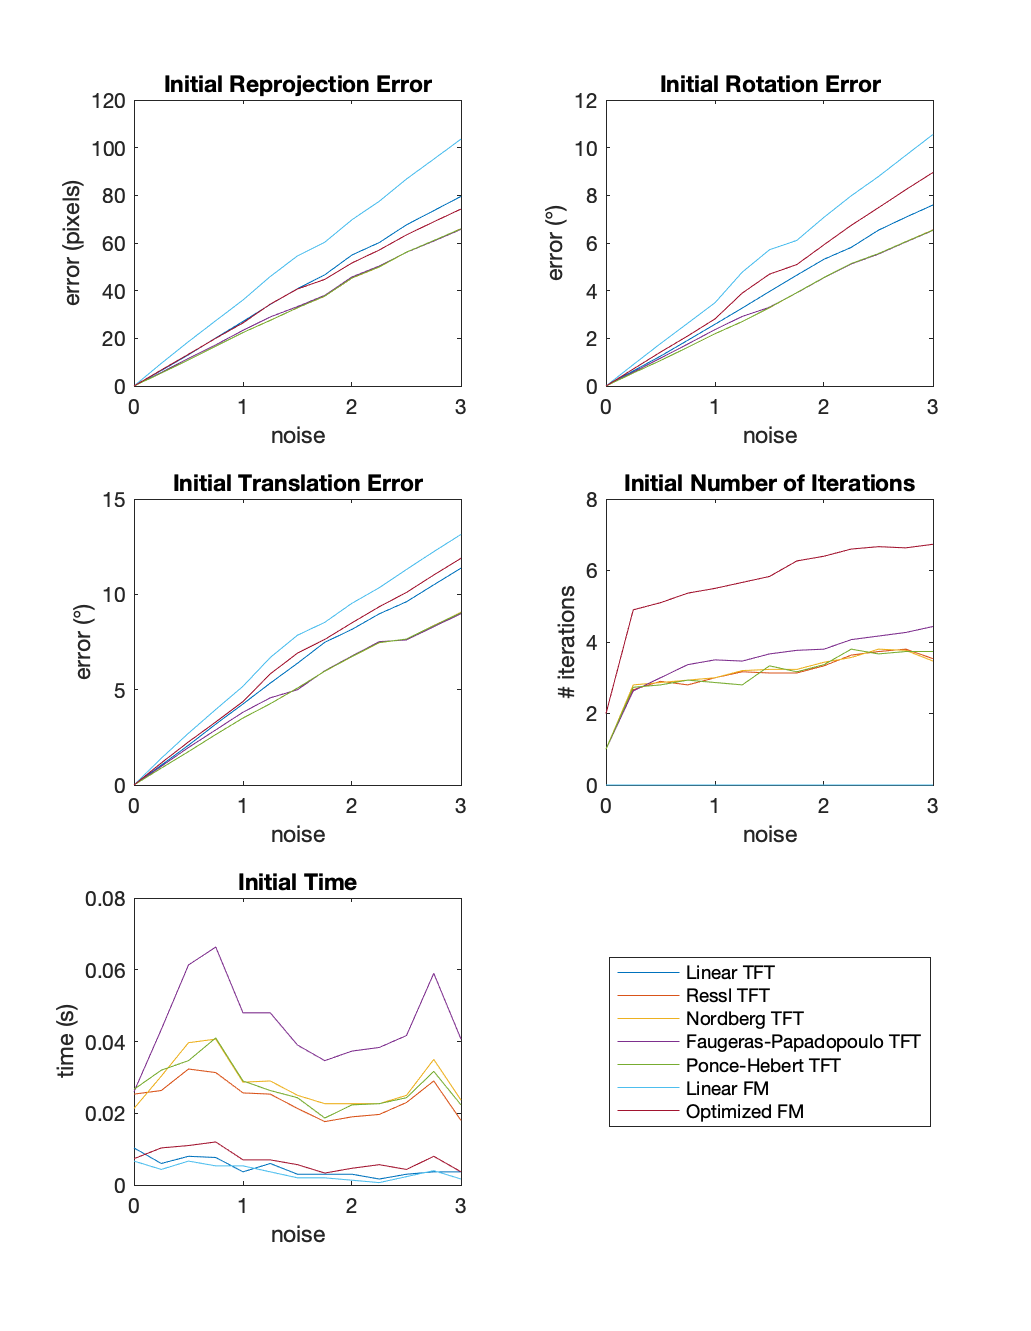
\includegraphics[width=1\textwidth]{Experiments/Synthetic/noise/INITnoisePlots.png}
	\caption{Initial reprojection error (top-left), rotation error (top-right), translation error (mid-left), number of iterations (mid-right), computational time (bottom-left); when varying the Gaussian noise added to the image points.}
	\label{fig:initNoisePlot}
\end{figure}

\begin{figure}[p]
	\centering
	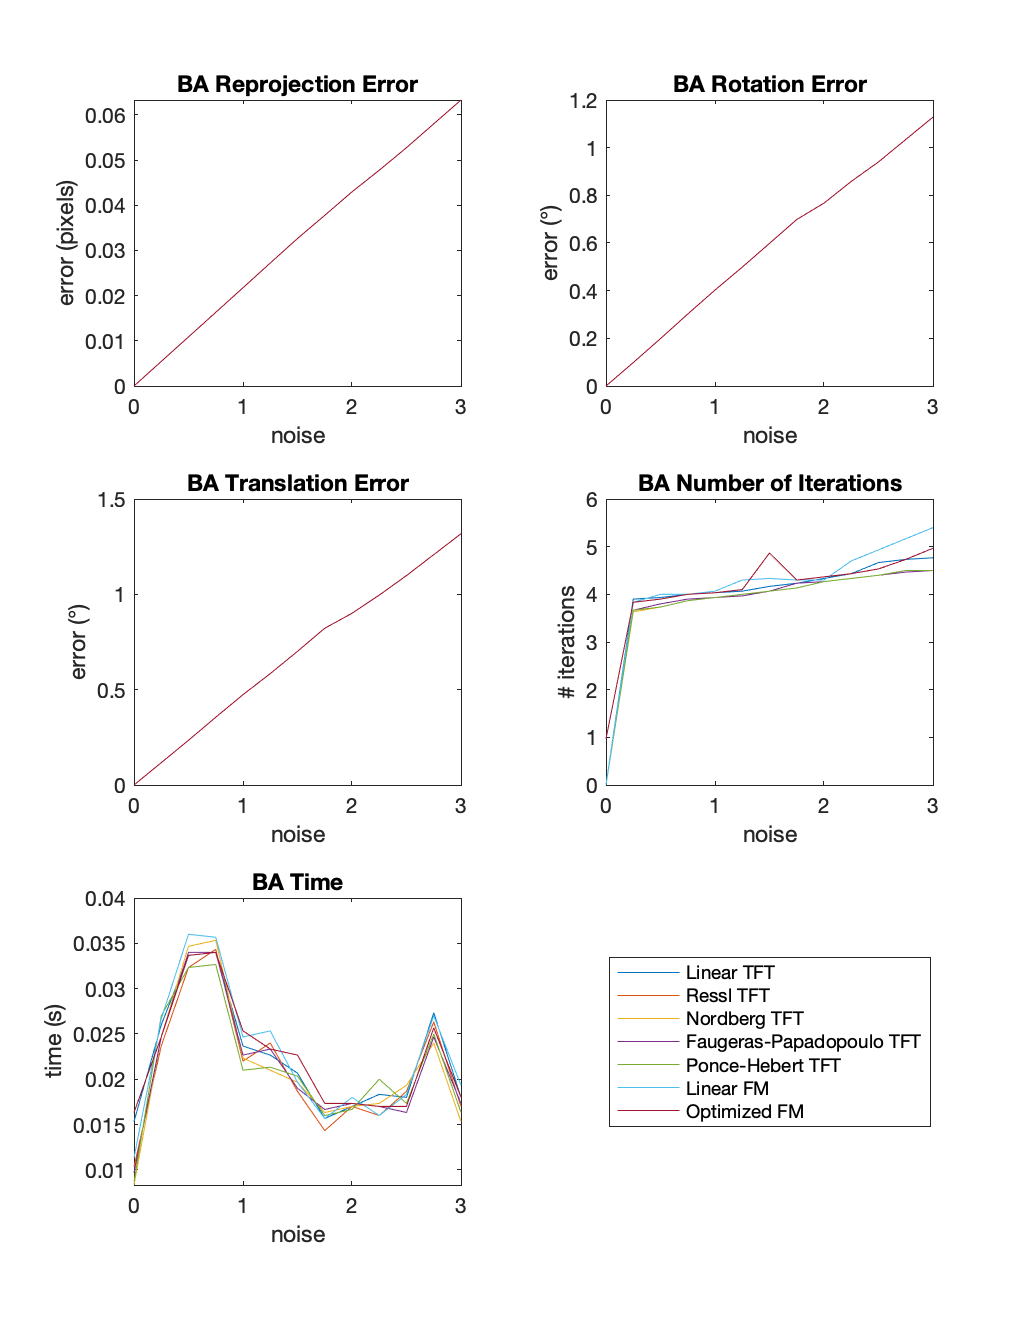
\includegraphics[width=1\textwidth]{Experiments/Synthetic/noise/BAnoisePlots.png}
	\caption{Reprojection error (top-left), rotation error (top-right), translation error (mid-left), number of iterations (mid-right), computational time (bottom-left) after Bundle Adjustment; when varying the focal length.}
	\label{fig:BANoisePlot}
\end{figure}

\pagebreak

Metrics before and after Bundle Adjustment, against Gaussian noise level added to the data points, is shown respectively in Figure (\ref{fig:initNoisePlot}) and Figure (\ref{fig:BANoisePlot}).

\begin{figure}[p]
	\centering
	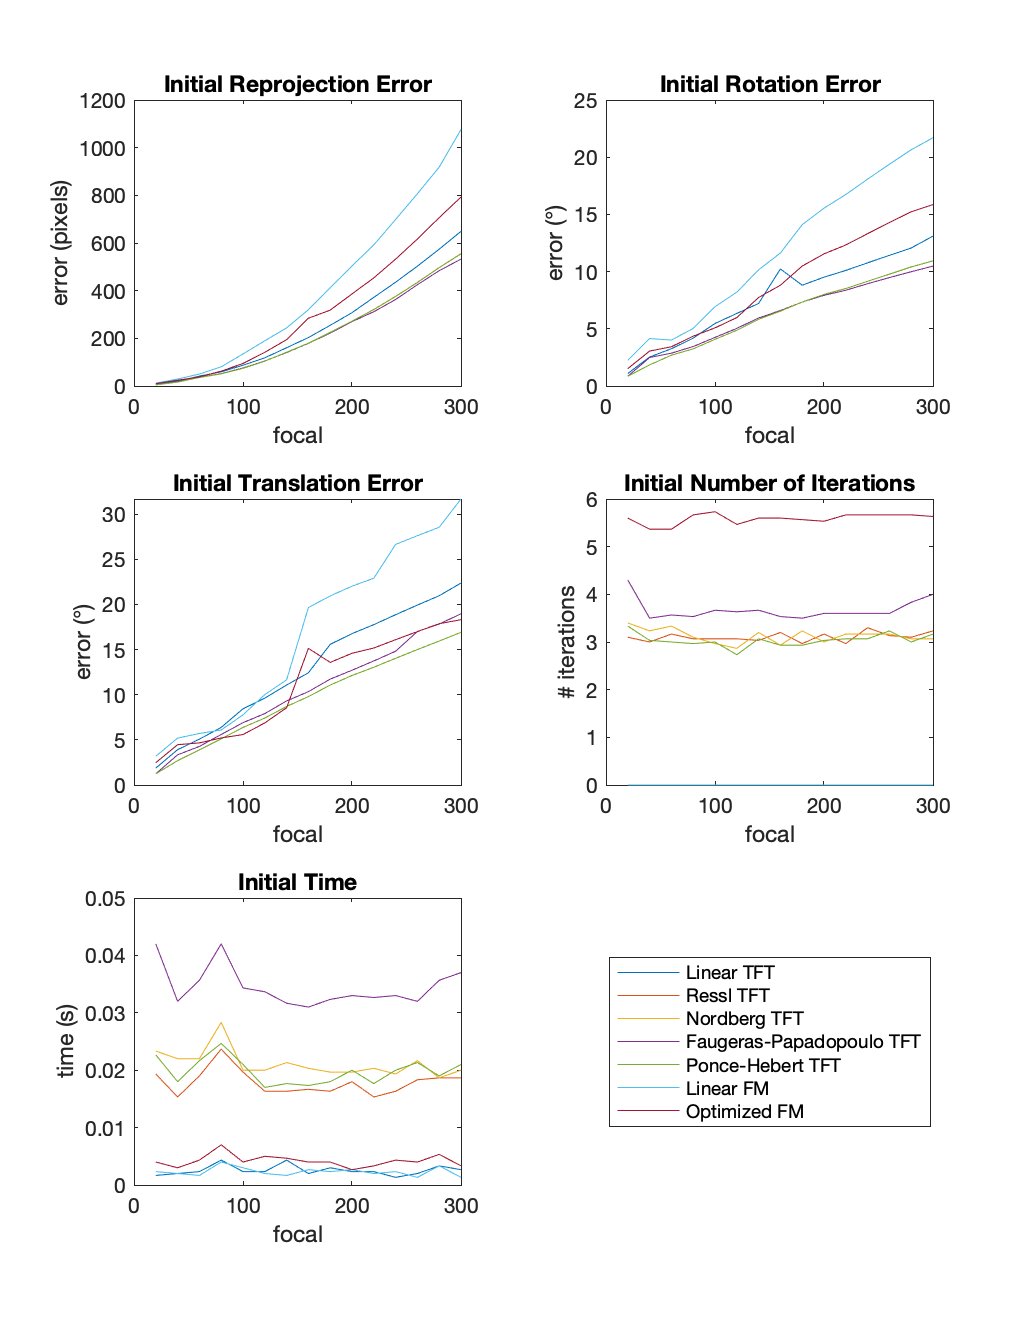
\includegraphics[width=1\textwidth]{Experiments/Synthetic/focal/INITfocalPlots.png}
	\caption{Initial reprojection error (top-left), rotation error (top-right), translation error (mid-left), number of iterations (mid-right), computational time (bottom-left); when varying the Gaussian noise added to the image points.}
	\label{fig:initFocalPlot}
\end{figure}

\begin{figure}[p]
	\centering
	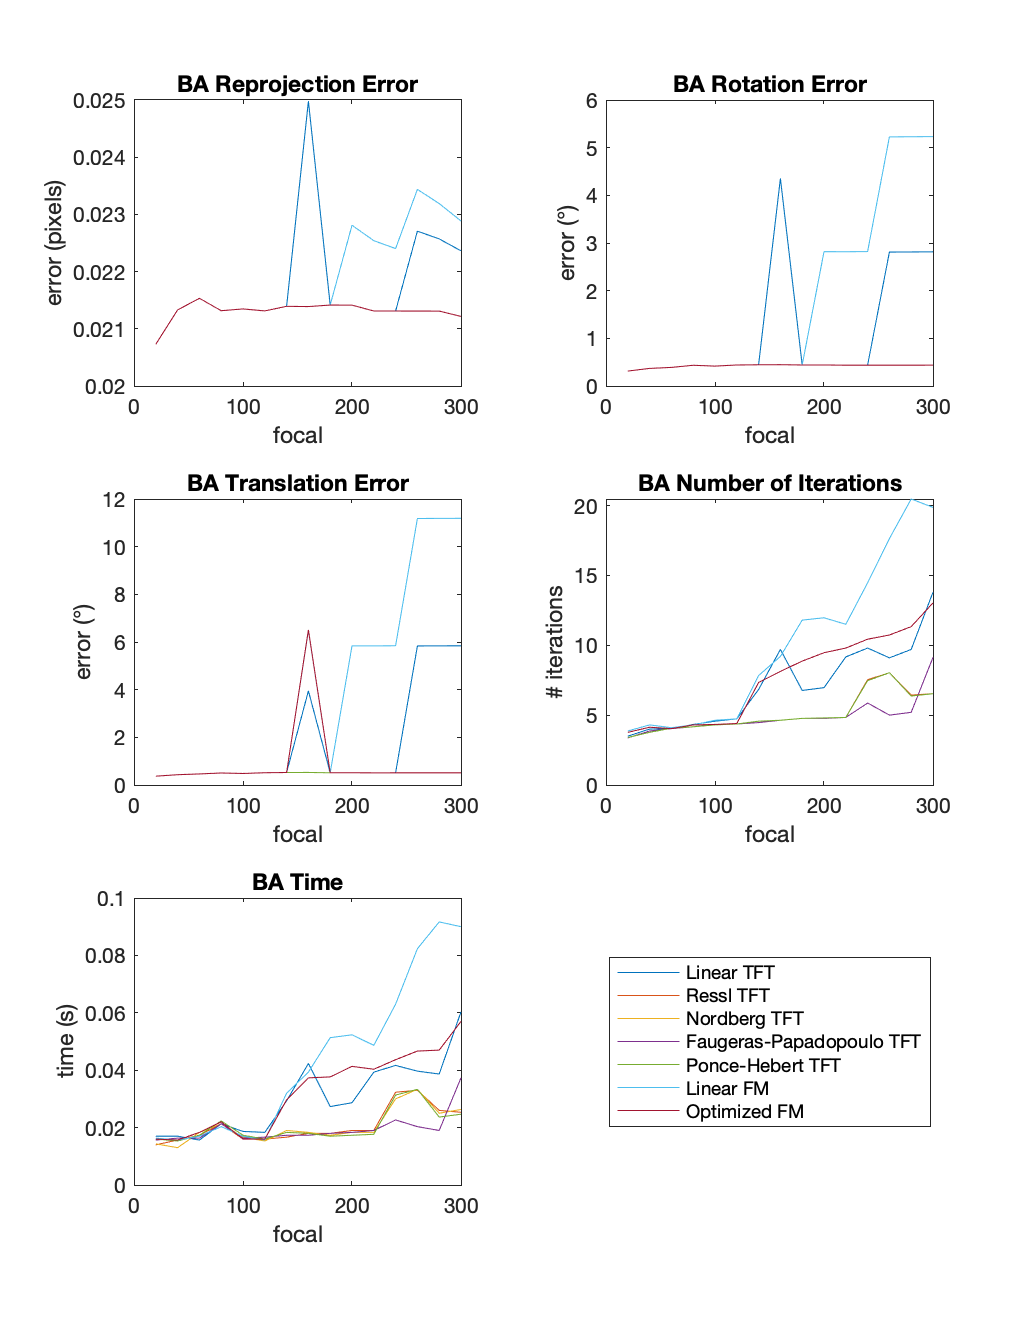
\includegraphics[width=1\textwidth]{Experiments/Synthetic/focal/BAfocalPlots.png}
	\caption{Reprojection error (top-left), rotation error (top-right), translation error (mid-left), number of iterations (mid-right), computational time (bottom-left) after Bundle Adjustment; when varying the focal length.}
	\label{fig:BAFocalPlot}
\end{figure}

\pagebreak

Metrics before and after Bundle Adjustment, against Gaussian noise level added to the data points, is shown respectively in Figure (\ref{fig:initFocalPlot}) and Figure (\ref{fig:BAFocalPlot}).

\begin{figure}[p]
	\centering
	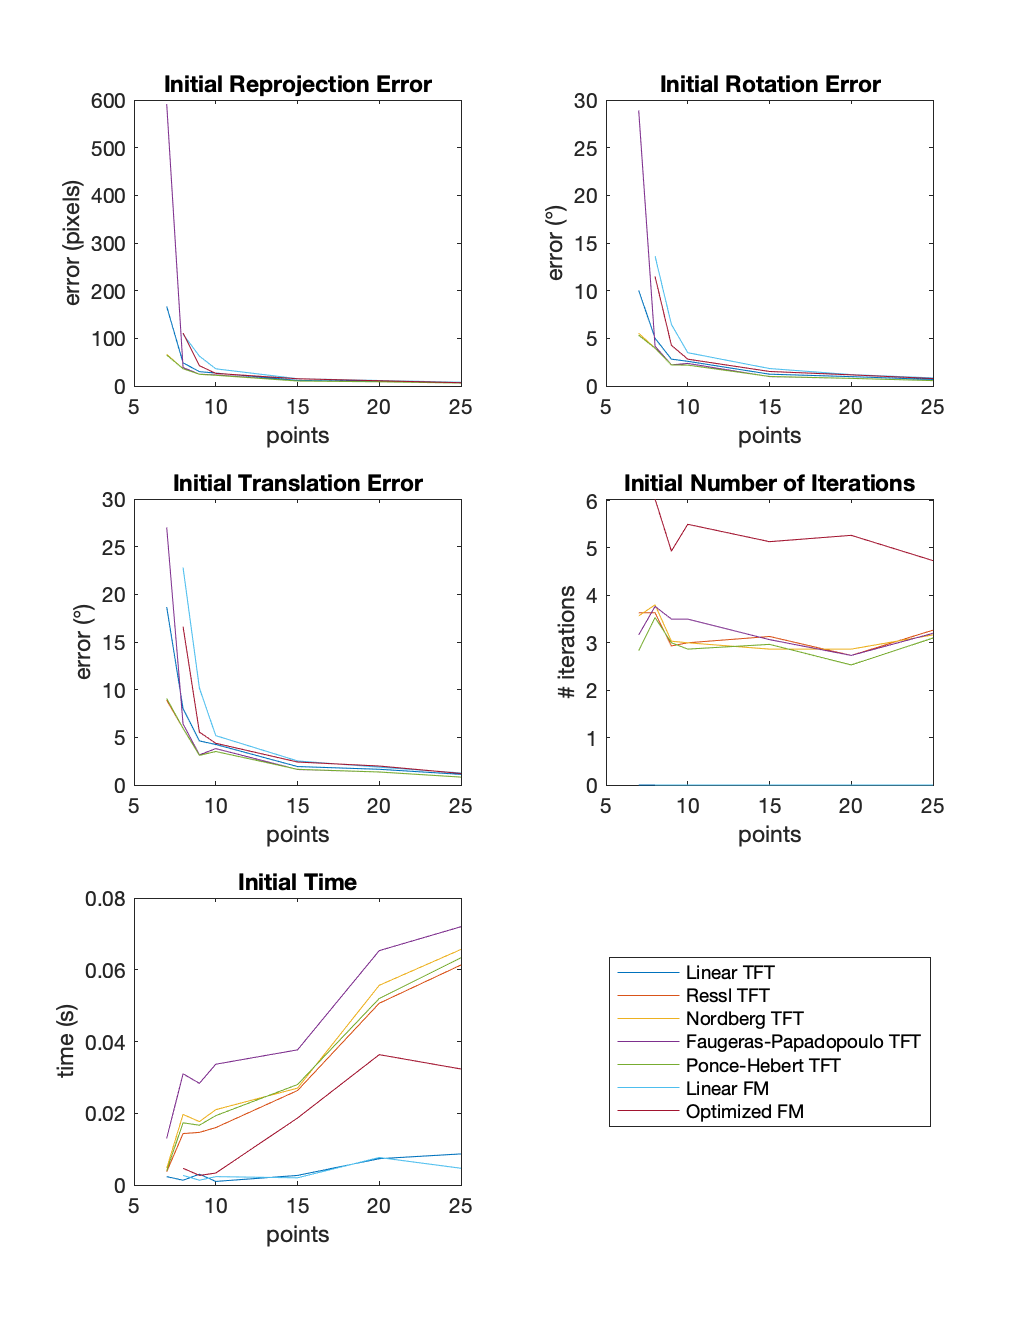
\includegraphics[width=1\textwidth]{Experiments/Synthetic/points/INITpointsPlots.png}
	\caption{Initial reprojection error (top-left), rotation error (top-right), translation error (mid-left), number of iterations (mid-right), computational time (bottom-left); when varying the number of image points.}
	\label{fig:initPointsPlot}
\end{figure}

\begin{figure}[p]
	\centering
	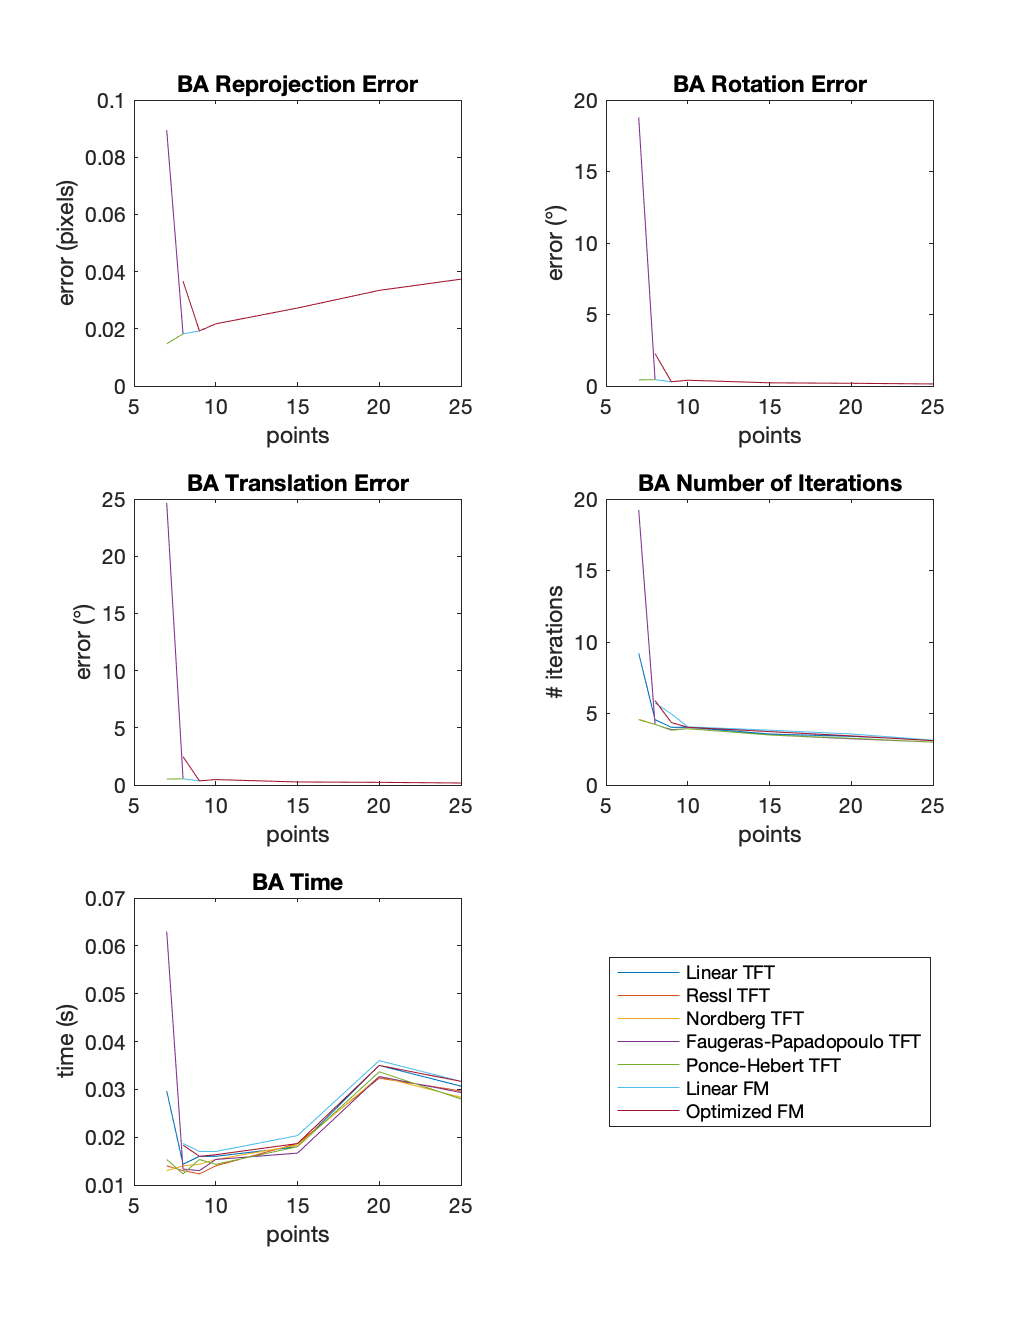
\includegraphics[width=1\textwidth]{Experiments/Synthetic/points/BApointsPlots.png}
	\caption{Reprojection error (top-left), rotation error (top-right), translation error (mid-left), number of iterations (mid-right), computational time (bottom-left) after Bundle Adjustment; when varying the number of image points.}
	\label{fig:BAPointsPlot}
\end{figure}

\pagebreak

Metrics before and after Bundle Adjustment, against Gaussian noise level added to the data points, is shown respectively in Figure (\ref{fig:initPointsPlot}) and Figure (\ref{fig:BAPointsPlot}).

\begin{figure}[p]
	\centering
	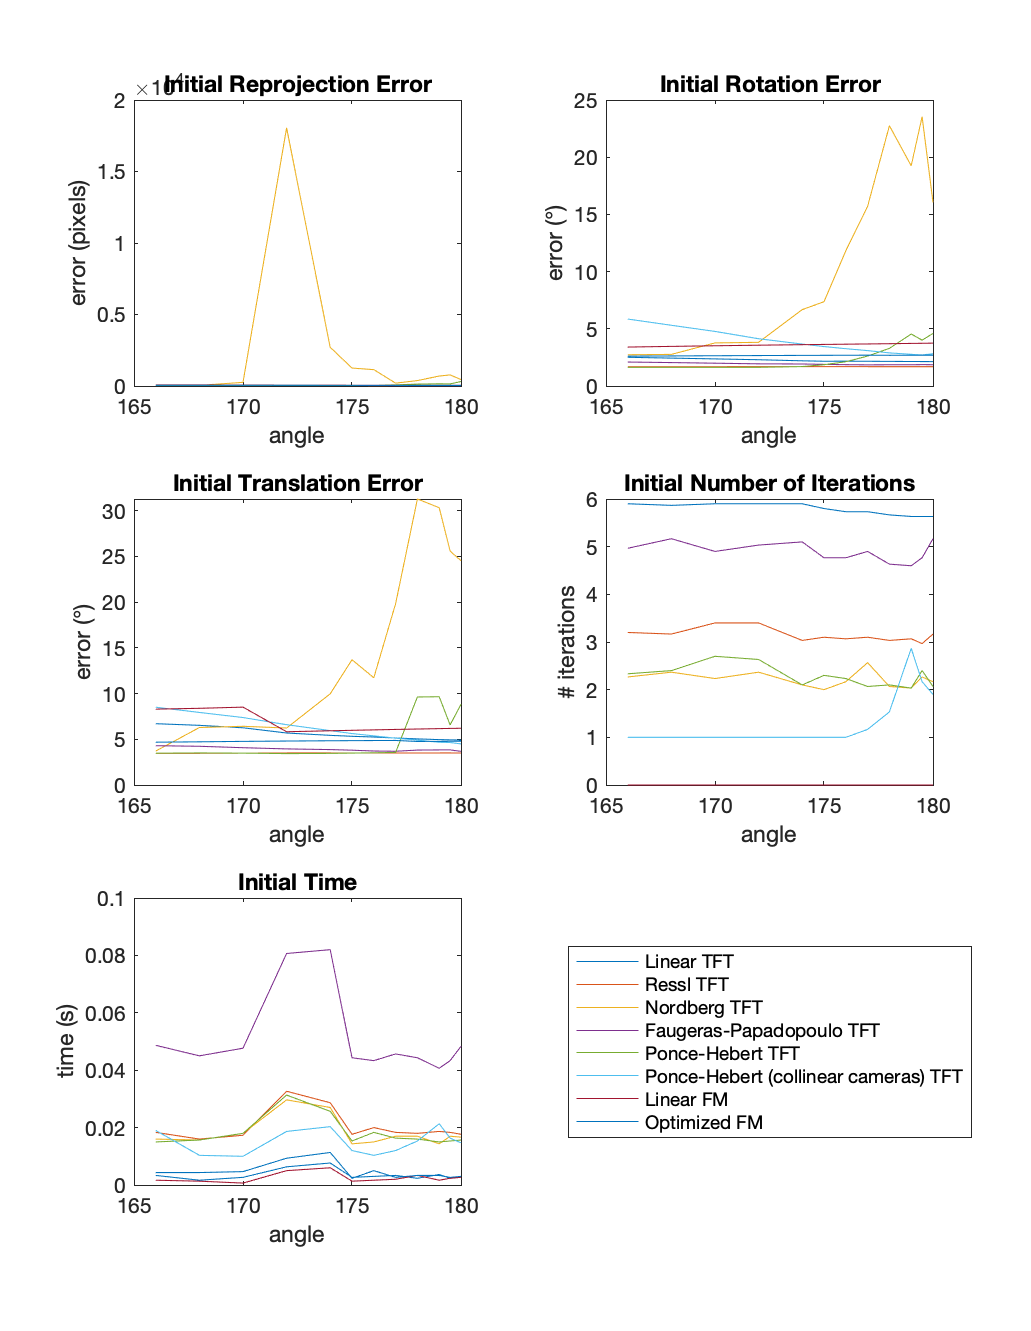
\includegraphics[width=1\textwidth]{Experiments/Synthetic/angle/INITanglePlots.png}
	\caption{Initial reprojection error (top-left), rotation error (top-right), translation error (mid-left), number of iterations (mid-right), computational time (bottom-left); when varying the angle among the three camera centers.}
	\label{fig:initAnglePlot}
\end{figure}

\begin{figure}[p]
	\centering
	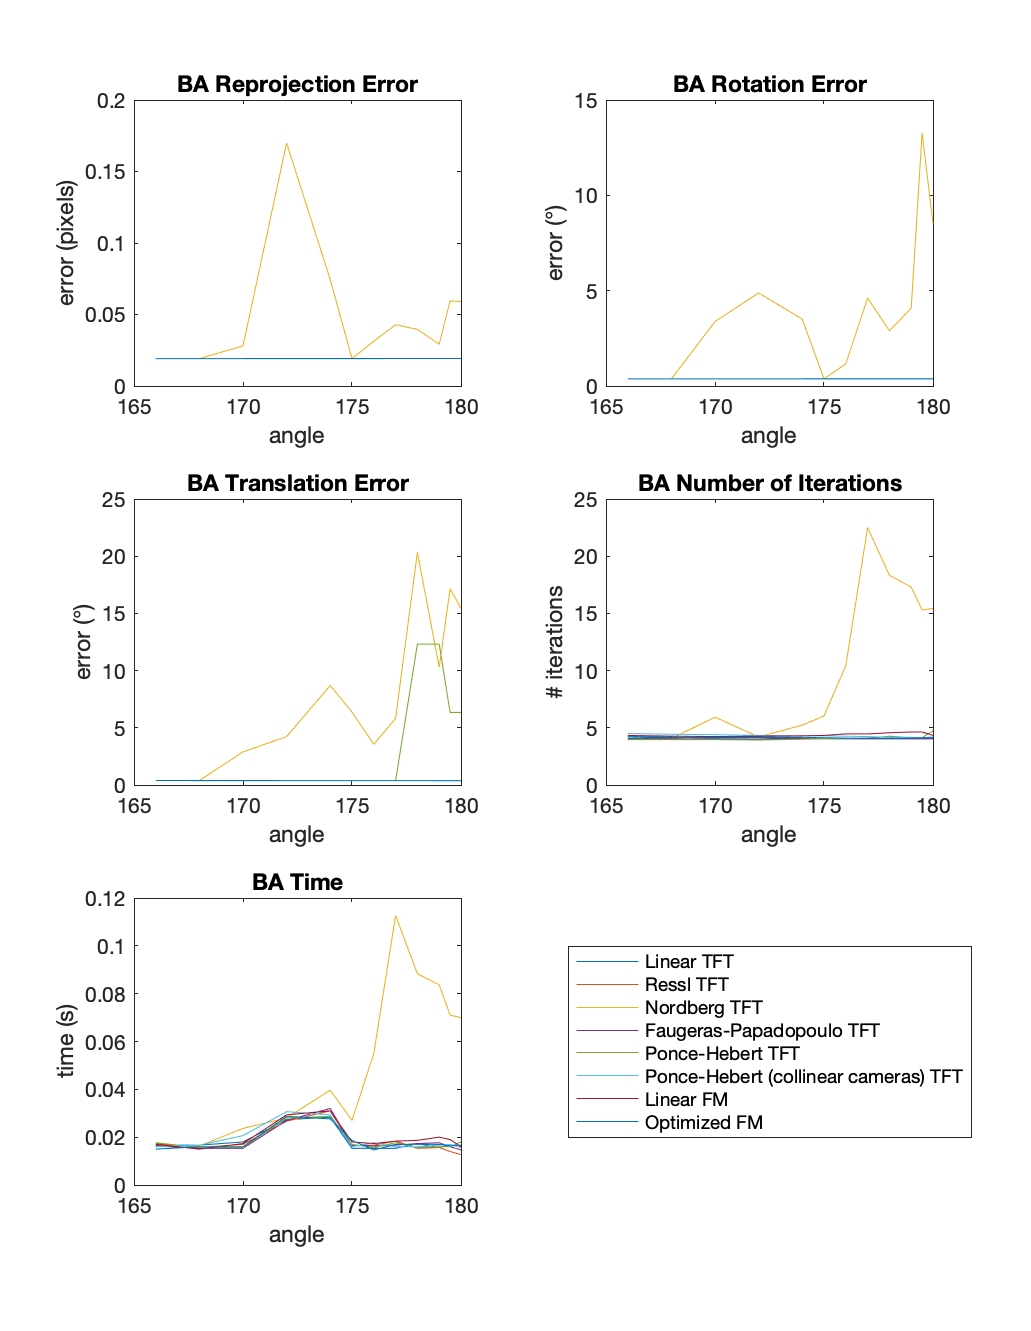
\includegraphics[width=1\textwidth]{Experiments/Synthetic/angle/BAanglePlots.png}
	\caption{Reprojection error (top-left), rotation error (top-right), translation error (mid-left), number of iterations (mid-right), computational time (bottom-left) after Bundle Adjustment; when varying the angle among the three camera centers.}
	\label{fig:BAAnglePlot}
\end{figure}

\pagebreak

Metrics before and after Bundle Adjustment, against Gaussian noise level added to the data points, is shown respectively in Figure (\ref{fig:initAnglePlot}) and Figure (\ref{fig:BAAnglePlot}).

\pagebreak

\subsection{Real Data}
In assessing the efficacy of these methods within real-world contexts, we opted to utilize scenes from the EPFL Dense Multi-View Stereo Dataset, presented in \cite{13-epfl-dataset}, provided by the CVLab at EPFL. \footnote{The EPFL Dense Multi-View Stereo Dataset comprising the utilized scenes is available at \href{https://documents.epfl.ch/groups/c/cv/cvlab-unit/www/data/multiview/denseMVS.html}{https://documents.epfl.ch/groups/c/cv/cvlab-unit/www/data/multiview/denseMVS.html}.}\\



\begin{table}[htbp]
  \centering
  \caption{Fountain Initial Data}
  \label{tab:fountainInit}
  \begin{tabular}{|*{6}{c}|}
    \hline
     & repr. error (px) & R error ($^{\circ}$) & t error ($^{\circ}$) & \# iter. & time (s)\\
    \hline
    Linear TFT & & & & & \\
    \hline
    Ressl TFT & & & & & \\
    \hline
    Faugeras-Papadopoulo TFT & & & & & \\
    \hline
    Ponce-Hebert TFT & & & & & \\
    \hline
    Linear FM & & & & & \\
    \hline
    Optimized FM & & & & & \\
    \hline
  \end{tabular}
\end{table}

\begin{table}[htbp]
  \centering
  \caption{Fountain after Bundle Adjustment}
  \label{tab:fountainBA}
  \begin{tabular}{|*{6}{c}|}
    \hline
     & repr. error (px) & R error ($^{\circ}$) & t error ($^{\circ}$) & \# iter. & time (s)\\
    \hline
    Linear TFT & & & & & \\
    \hline
    Ressl TFT & & & & & \\
    \hline
    Faugeras-Papadopoulo TFT & & & & & \\
    \hline
    Ponce-Hebert TFT & & & & & \\
    \hline
    Linear FM & & & & & \\
    \hline
    Optimized FM & & & & & \\
    \hline
  \end{tabular}
\end{table}

\begin{table}[htbp]
  \centering
  \caption{HerzJesu Initial Data}
  \label{tab:HerzJesuInit}
  \begin{tabular}{|*{6}{c}|}
    \hline
     & repr. error (px) & R error ($^{\circ}$) & t error ($^{\circ}$) & \# iter. & time (s)\\
    \hline
    Linear TFT & & & & & \\
    \hline
    Ressl TFT & & & & & \\
    \hline
    Faugeras-Papadopoulo TFT & & & & & \\
    \hline
    Ponce-Hebert TFT & & & & & \\
    \hline
    Linear FM & & & & & \\
    \hline
    Optimized FM & & & & & \\
    \hline
  \end{tabular}
\end{table}

\begin{table}[htbp]
  \centering
  \caption{HerzJesu after Bundle Adjustment}
  \label{tab:HerzJesuBA}
  \begin{tabular}{|*{6}{c}|}
    \hline
     & repr. error (px) & R error ($^{\circ}$) & t error ($^{\circ}$) & \# iter. & time (s)\\
    \hline
    Linear TFT & & & & & \\
    \hline
    Ressl TFT & & & & & \\
    \hline
    Faugeras-Papadopoulo TFT & & & & & \\
    \hline
    Ponce-Hebert TFT & & & & & \\
    \hline
    Linear FM & & & & & \\
    \hline
    Optimized FM & & & & & \\
    \hline
  \end{tabular}
\end{table}
